\documentclass[a4paper]{article}

% CJK support: prefer ctex, fallback to XeTeX native line breaking
\IfFileExists{ctex.sty}{
  \usepackage[fontset=fandol]{ctex}
}{
  % Fallback for minimal TeX installs (e.g. MacTeX Basic, TeX Live scheme-basic)
  % without ctex/xeCJK. Uses XeTeX's built-in CJK line breaking.
  \usepackage{fontspec}
  \XeTeXlinebreaklocale "zh"
  \XeTeXlinebreakskip = 0pt plus 1pt
  \IfFontExistsTF{Songti SC}{\setmainfont{Songti SC}}{%
    \IfFontExistsTF{Noto Serif CJK SC}{\setmainfont{Noto Serif CJK SC}}{}%
  }
  \IfFontExistsTF{Heiti SC}{\setsansfont{Heiti SC}}{%
    \IfFontExistsTF{Noto Sans CJK SC}{\setsansfont{Noto Sans CJK SC}}{}%
  }
}

% Basic packages
\usepackage{amsmath, amssymb}
\usepackage{graphicx}
\usepackage[margin=2.5cm]{geometry}
\usepackage[most]{tcolorbox}
\usepackage{etoolbox}
\usepackage{listings}
\usepackage{hyperref}
\usepackage{booktabs}
\usepackage{subcaption}
\usepackage{float}
\usepackage{tikz}
\IfFileExists{pgfplots.sty}{
    \usepackage{pgfplots}
    \pgfplotsset{compat=1.18}
}{}

% ===== Highlight boxes =====
\newtcolorbox{knowledgebox}[1]{
    enhanced, colback=blue!5!white, colframe=blue!75!black, colbacktitle=blue!75!black,
    coltitle=white, fonttitle=\bfseries, title=#1, attach boxed title to top left={yshift=-2mm, xshift=2mm},
    boxrule=1pt, sharp corners
}

\newtcolorbox{importantbox}[1]{
    enhanced, colback=yellow!10!white, colframe=yellow!80!black, colbacktitle=yellow!80!black,
    coltitle=black, fonttitle=\bfseries, title=#1, sharp corners
}

\newtcolorbox{warningbox}[1]{
    enhanced, colback=red!5!white, colframe=red!75!black, colbacktitle=red!75!black,
    coltitle=white, fonttitle=\bfseries, title=#1, sharp corners
}

% ===== Code listings =====
\lstset{
    basicstyle=\ttfamily\small,
    keywordstyle=\color{blue},
    stringstyle=\color{red!60!black},
    commentstyle=\color{green!60!black},
    breaklines=true,
    frame=single,
    numbers=left,
    numberstyle=\tiny\color{gray},
    captionpos=b,
    extendedchars=false
}

% ===== Figure provenance and unit macros =====
% \vtag goes inside \caption{...}; \srcnote{MM:SS--MM:SS} follows the figure environment.
\newcommand{\vtag}{\protect\footnotemark}
\newcommand{\srcnote}[1]{\footnotetext{视频画面时间区间：#1。若为裁剪图，时间区间仍对应原视频画面。}}
% Units work in text and math mode; never hand-write $^\circ$ or \AA inside \mathrm.
\newcommand{\degC}{\ensuremath{^{\circ}\mathrm{C}}}
\newcommand{\um}{\ensuremath{\mu\mathrm{m}}}
\newcommand{\nm}{\ensuremath{\mathrm{nm}}}
\newcommand{\angstrom}{\ensuremath{\text{\AA}}}

% ===== Front-page metadata =====
% Fill these in when generating notes.
\newcommand{\notetitle}{需求和架构（二）}
\newcommand{\notesubtitle}{南京大学《生成式软件工程》2026 秋季 · 第 7 讲}
\newcommand{\noteauthors}{讲者：蒋炎岩 · 整理：lecture-to-notes}
\newcommand{\notedate}{2026 年 10 月 3 日}
\newcommand{\videochannel}{绿导师原谅你了}
\newcommand{\videopublishdate}{2026 年 9 月 29 日}
\newcommand{\videoduration}{99 分 41 秒}
\newcommand{\videourl}{https://www.bilibili.com/video/BV1JGap6LE74/}
\newcommand{\videocoverpath}{cover.jpg}

\hypersetup{pdftitle={南京大学生成式软件工程第7讲：需求和架构（二）},pdfauthor={lecture-to-notes},colorlinks=true,linkcolor=blue!45!black,urlcolor=blue!60!black}
\setlength{\parskip}{0.4em}
\setlength{\emergencystretch}{2em}
\begin{document}

% ===== Title page =====
\begin{titlepage}
\centering
{\Large 课程笔记\par}
\vspace{1.2cm}
{\huge\bfseries \notetitle\par}
\ifdefempty{\notesubtitle}{}{
\vspace{0.3cm}
{\large \notesubtitle\par}
}
\vspace{0.5cm}
{\large \noteauthors\par}
\vspace{0.3cm}
{\large \notedate\par}
\vspace{1.0cm}

\ifdefempty{\videocoverpath}{
{\small 请在生成笔记时填入视频封面图的本地路径。\par}
}{
\includegraphics[width=0.82\textwidth,height=0.40\textheight,keepaspectratio]{\videocoverpath}\par
}

\vfill
\begin{tcolorbox}[width=0.9\textwidth, colback=black!2!white, colframe=black!60, sharp corners]
\textbf{视频作者/频道}：\videochannel\par
\textbf{发布日期}：\videopublishdate\par
\textbf{视频时长}：\videoduration\par
\textbf{视频链接}：
\ifdefempty{\videourl}{
未填写
}{
\href{\videourl}{\nolinkurl{\videourl}}
}
\end{tcolorbox}
\end{titlepage}

\tableofcontents
\newpage

\section{需求与架构怎样共同控制复杂性}
\label{sec:complexity}
一个软件可以完全满足今天列出的功能，却在下一轮修改中陷入维护泥潭。本讲要回答的是：当需求、业务规则和技术环境继续变化时，怎样让已经做出的决定仍有容纳变化的空间？讲者从需求与架构的边界出发，追溯结构化程序设计和可生长语言的思想，再用 UNIX、数据库、网络、界面框架及记账系统说明它们怎样落到具体实现中。

阅读这份笔记只需要基础编程知识。读完后，应能辨别一个复杂问题究竟来自业务本身，还是来自实现组织方式；也应能沿着一项变化，指出它影响哪些模块、哪些状态，以及这些影响怎样计算和查证。全文按理解所需的先后顺序重组课堂材料，图下注明原视频时间。课堂中的评价和预测保留讲者归属，笔记的归纳会明确标出。

\subsection{意图、规约和实现之间都有选择}
意图说明想达到的目标，规约明确允许和禁止的行为，实现决定怎样执行这些行为。三者之间都有多种可能的映射。选课系统的意图是公平分配稀缺名额，但公平可以解释成同优先级随机抽签，也可以解释成按需求强度排序；即使选择抽签，系统仍要决定什么时候触发、怎样存储结果，以及怎样处理候补。

图中不同的分支说明，需求描述并不会自动唯一确定程序。一个未经确认的假设，可以在后面的设计中变成默认规则，再逐步偏离原来的目标。生成代码的速度越快，越需要在有影响的分叉处停下来，确认这个决定究竟出自客户、讲者提出的方案，还是实现者自己的猜测。
\begin{figure}[H]
\centering
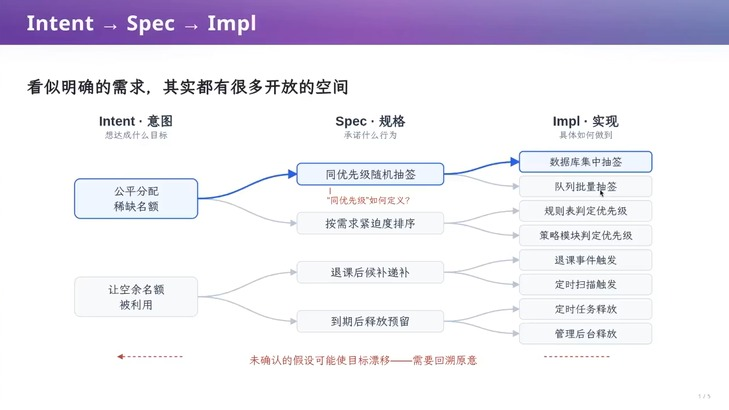
\includegraphics[width=\textwidth]{figures/fig_01_intent_spec_impl.jpg}
\caption{意图、规约和实现中的开放选择\vtag}
\end{figure}
\srcnote{00:00:22--00:00:30}

架构并不只属于几十万行的系统。上一讲的约十行汉诺塔、约 20,000 行二维码工具和约 500,000 行教务系统，都面临表示、操作以及接口的选择。这些数字是课堂用来说明规模跨度的例子，不是架构复杂度的计量公式。一个小程序也可能因表示选择而难以调试，一个大系统也可能依靠合适的抽象使局部保持清楚。
\begin{figure}[H]
\centering
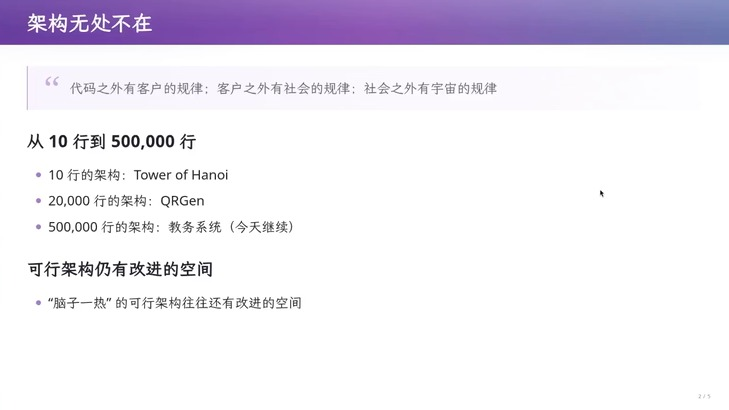
\includegraphics[width=\textwidth]{figures/fig_02_architecture_everywhere.jpg}
\caption{从十行程序到教务系统的架构\vtag}
\end{figure}
\srcnote{00:01:07--00:01:15}

\subsection{业务要求的复杂性与实现制造的复杂性}
本质复杂性来自问题领域。课程容量、先修要求、上课时间冲突以及教室借用，都是现实工作中的约束。把软件换成人工办理，这些问题仍然存在。附带复杂性来自实现方式：重复保存数据、转换格式、同步缓存、配置部署，以及因某种技术选型而新增的中间层。
\begin{figure}[H]
\centering
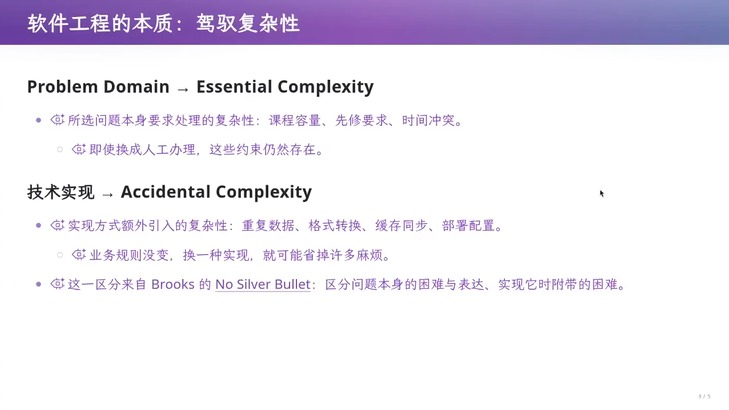
\includegraphics[width=\textwidth]{figures/fig_03_essential_accidental.jpg}
\caption{本质复杂性与附带复杂性\vtag}
\end{figure}
\srcnote{00:03:37--00:03:45}

课堂用文件系统与数据库说明取舍。文件容易直接检查和修改，也容易接入 UNIX 工具；数据库则提供事务等数据管理能力。需要把一组读写作为整体处理时，仅靠普通文件读写并不会自动得到数据库事务的保证。使用数据库又会增加查询和调试的间接层。架构选择需要比较它解决了哪些困难、又引入了哪些困难，而不能只问某个技术是否流行。

\begin{importantbox}{识别复杂性的办法}
先问：如果不用计算机，这个约束还存在吗？仍然存在的课程容量和先修条件属于领域问题；多份数据必须手工同步，则应继续追问是否是实现方式造成的。这个问题帮助找出改进方向，不表示两种复杂性在任何场景里都能截然分开。
\end{importantbox}

\subsection{澄清需求会减少猜测，也增加承诺}
“课程容量为 100 人”需要继续确认：候补是否计入，跨院预留名额是否可以借用。约束越清楚，实现者自行决定的空间越小。但每条需求也都需要审计和维护；在生成式开发中，它还占用上下文和 token，并增加复杂约束交互时的出错机会。
\begin{figure}[H]
\centering
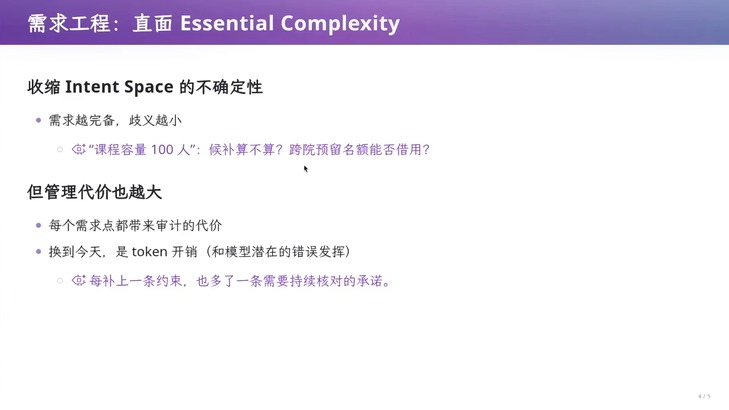
\includegraphics[width=\textwidth]{figures/fig_04_requirements_uncertainty.jpg}
\caption{需求澄清与约束维护的代价\vtag}
\end{figure}
\srcnote{00:06:07--00:06:15}

登录是课堂的另一例子。一句“需要登录”可能被模型展开为自建用户名和密码，再连带出现注册、密码确认、忘记密码、发邮件或短信的需求。接入第三方身份服务又会带来服务资格、责任与费用方面的取舍。这里的重点是识别由一个选择衍生出的整串承诺，不是推荐某一种现成认证方案。

讲者把快速做最小可行产品与广度上的决策比较放在一起。先做一条可体验的路径，能验证核心功能是否满足意图；同时仍要审视认证方式、首页布局等关键分叉，避免把第一次能运行的方案当作唯一答案。原型验证与设计思考应相互提供信息。

\subsection{架构给变化建立边界}
架构分解不能消除的业务问题，并减少实现额外制造的麻烦。容量、资格和冲突检查可以各有明确职责，但普通选课、管理员补选和批量导入，应复用适用的共同规则。数据归属、接口和模块责任明确后，大量随意组合的实现方式就被排除。
\begin{figure}[H]
\centering
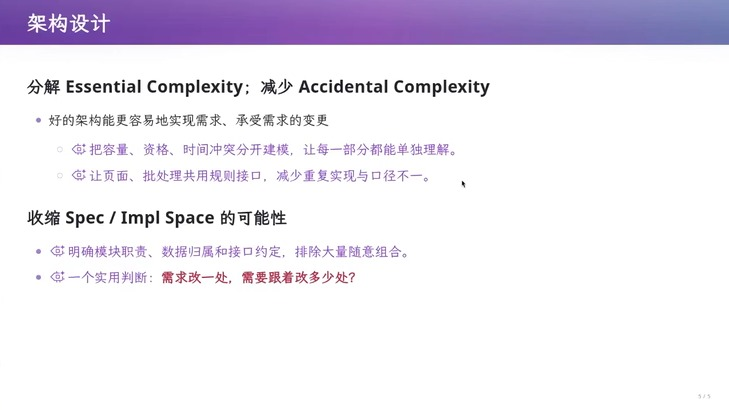
\includegraphics[width=\textwidth]{figures/fig_05_architecture_boundaries.jpg}
\caption{分解复杂性并限制实现组合\vtag}
\end{figure}
\srcnote{00:11:37--00:11:45}

\begin{knowledgebox}{一个实用的架构问题}
需求改一处，系统里要改多少处？这个提问关注同一个业务决定传播了多远。修改点数量不能单独证明架构好坏，但规则在多个入口中重复出现，通常说明应检查职责和依赖的组织方式。
\end{knowledgebox}

\subsection{本章小结}
需求工程澄清想要什么，架构设计限制怎样实现，并给后续变化安排位置。两者都需要作决定，也都会承担决定之后的维护成本。要理解为什么分解和接口如此关键，还要回到一个更基础的限制：人的头脑不能同时精确追踪整个系统。

\section{有限的头脑怎样理解更大的程序}
\label{sec:abstraction}
抽象的价值，是让使用者在某一层只处理少量有意义的概念，同时有条件地依赖下一层的承诺。它不会抹掉细节，却能避免每次操作都把所有细节一起展开。课堂借 1972 年的《Structured Programming》说明，这个问题早于今天的框架，也没有因工具变强而消失。

\subsection{尊重注意力的边界}
讲者引用 Dijkstra 对自身理解能力的反思：程序员应承认同时处理的信息有限，并据此构造程序。今天看来很小的顺序、选择、循环程序，仍然能展示这种思路。层次化分解的目的，是把不能一次理解的整体，变成能够逐层理解、逐层检查的结构。
\begin{figure}[H]
\centering
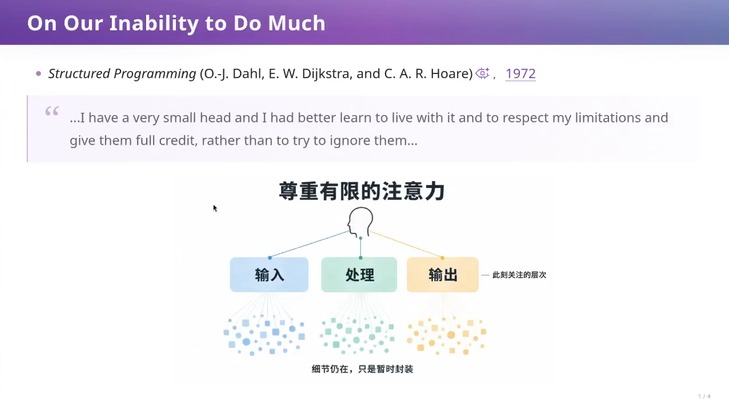
\includegraphics[width=\textwidth]{figures/fig_06_small_head.jpg}
\caption{有限注意力与程序层次\vtag}
\end{figure}
\srcnote{00:14:37--00:14:45}

\begin{importantbox}{抽象需要可依赖的承诺}
调用者知道某个操作的条件、效果和限制，才有理由暂时不展开实现。若模块名字听起来清楚，但调用者仍必须知道它的全部内部数据与控制顺序，这个名字就没有完成隔离复杂性的工作。
\end{importantbox}

\subsection{枚举、归纳与抽象各有什么作用}
枚举让人检查有限的分支；归纳让人理解循环与递归中的重复结构；抽象让人用一个概念代替一组已经理解的操作。这三种思维辅助相互配合：先把一个局部的含义说清楚，再利用它处理更大的结构，而不是在脑中逐条展开全部执行过程。
\begin{figure}[H]
\centering
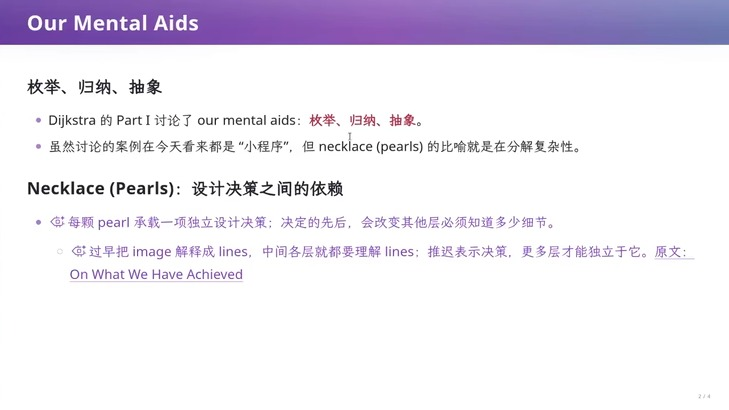
\includegraphics[width=\textwidth]{figures/fig_07_mental_aids.jpg}
\caption{枚举归纳抽象与珍珠项链\vtag}
\end{figure}
\srcnote{00:21:07--00:21:15}

珍珠项链的比喻强调设计决定之间的依赖。每一颗珍珠承担一项决定，串联关系决定上层能够使用什么。决定顺序会影响多少后续层必须理解某个细节。例如，过早把图像解释成一行行数据，中间层便都要认识“行”；如果暂缓这个表示决定，更多层就可以继续围绕“图像”这个概念工作。可替换性取决于共同承诺是否保持，而不只取决于程序切出了多少块。

\subsection{对象与协程分解不同种类的耦合}
类和对象把相关的数据与操作包装成一个概念。SIMULA 中的概念层次使使用者可以从问题领域出发，再逐层落到机器操作。协程则处理控制流的耦合：子程序服从调用与返回，协程可以暂停、保留自己的执行位置，之后再恢复。
\begin{figure}[H]
\centering
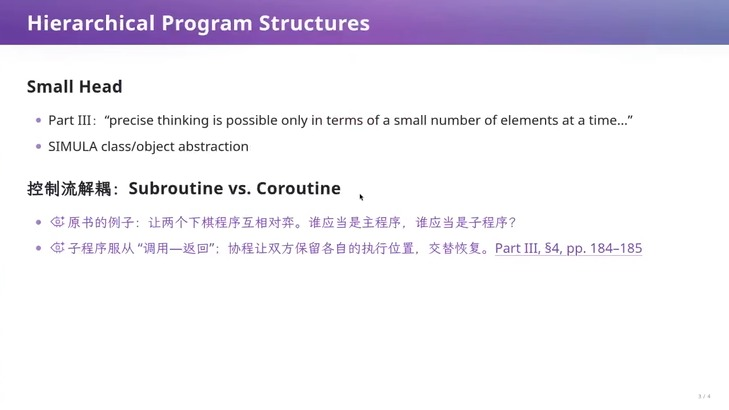
\includegraphics[width=\textwidth]{figures/fig_08_hierarchical_coroutine.jpg}
\caption{对象抽象与协程控制流解耦\vtag}
\end{figure}
\srcnote{00:24:37--00:24:45}

两个下棋程序交替行动，双方都要算一步、交给对方、等待回应、继续执行。强行把一方改成另一方的子程序，会改变原本对等的程序组织；让双方分别保留自己的执行位置，则更贴近这种合作结构。课堂将这个历史动机与今天为降低调度开销而使用的协程联系起来，但没有把所有现代协程机制都等同于 SIMULA 的实现。

\begin{knowledgebox}{控制流也是架构的一部分}
分解数据不等于分解控制。既要问“哪些状态属于同一个概念”，也要问“哪些流程需要独立记住自己做到哪一步”。对象与协程为这两个问题提供了不同的组织工具。
\end{knowledgebox}

\subsection{从链表操作长出车间模拟的词汇}
课堂推荐沿第三部分第七节的原文阅读：TWLIST 提供双向链表操作，MINISIM 在其上组织离散事件模拟，Job Shop Model 再描述订单与机器。课件给出的阅读范围是原文 208--220 页；协程案例位于第三部分第四节的 184--185 页。
\begin{figure}[H]
\centering
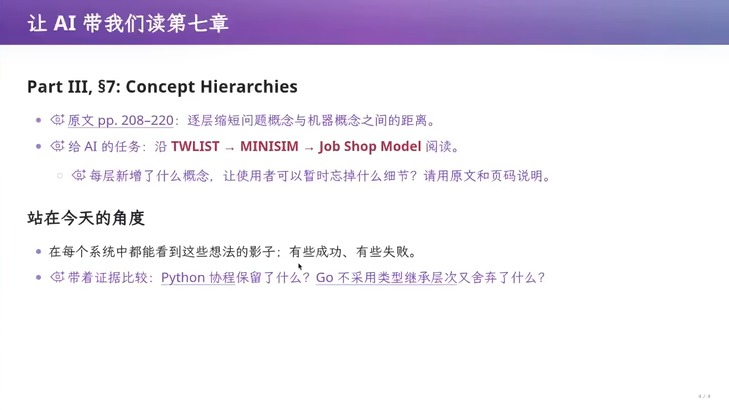
\includegraphics[width=\textwidth]{figures/fig_09_concept_hierarchy.jpg}
\caption{TWLIST到MINISIM再到车间模型\vtag}
\end{figure}
\srcnote{00:33:37--00:33:45}

底层管理连接关系，中层管理模拟时间、等待与唤醒，上层便能表达请求机器、加工、释放资源。\texttt{hold}、\texttt{activate}、\texttt{simulate} 等操作让模拟者使用领域相关的动作，而不必反复手工维护底层执行过程。这里值得学习的是每一层新增了什么能力、隐藏了什么细节，以及它要求调用者遵守什么条件。

\subsection{动态规划也可以有一个小架构}
讲者用难调试的动态规划说明，小程序也会失去清晰的概念层。若代码只剩 \texttt{dp[i][j][k]} 和若干循环，状态的业务或数学含义便容易被数组下标淹没。一处转移写错，不一定崩溃，可能只悄悄得到错误结果。

课堂建议把状态及其迁移的概念放回来：给状态命名，能查询它有哪些后继，能打印或可视化相邻状态与迁移。在课堂所讨论的有向无环状态空间里，读者便能用问题本身的结构理解计算。调试清楚后，再改写为等价而更高效的数组形式。讲者没有主张所有动态规划都使用同一封装，而是提示表示方式应服务于理解和检查。

\subsection{让 AI 带读，也要回到原文}
讲者把 AI 用作寻找、翻译和解释经典材料的助手，并将 1980 年到 2010 年称为自己关注领域的一段黄金时期。这是他的阅读经验与评价，不是关于全部计算机研究的客观分期。课堂还展示了收集大量论文、核对列表和围绕原文追问的方式。

有效问题应具体到层次：“新引入了什么概念？”“调用者因此不用关心什么？”“原文哪段代码支持这个解释？”模型给出一个现代对应物，并不等于已经证明两个机制相同。带着代码和页码核对，才能使模型的概括进入自己的知识结构。

\subsection{本章小结}
抽象、层次和独立控制流，帮助有限的头脑分批理解程序。它们还有更长远的作用：已经定义好的概念可以成为未来设计的材料。接下来要问，架构怎样使这些材料继续组合，而不把未来用途全部预先固定。

\section{好的架构怎样留下未来的解空间}
\label{sec:growth}
可生长架构提供一组有含义的原语及组合规则，使后来的使用者能构造设计者没有逐项列出的用途。这样的设计需要同时考虑今天固定什么、以后开放什么，以及不同扩展是否仍能共同工作。

\subsection{名字承载已经理解的概念}
课堂从 Guy L. Steele Jr. 在 SICP 前言中的命名观点出发。一个名字可以唤起已经建立的知识，使人用队列、事务或选课资格思考，而不必每次重新展开内部细节。Steele 参与 Scheme、Common Lisp 和 Java 相关设计，这些经历为后面讨论语言的生长提供背景。
\begin{figure}[H]
\centering
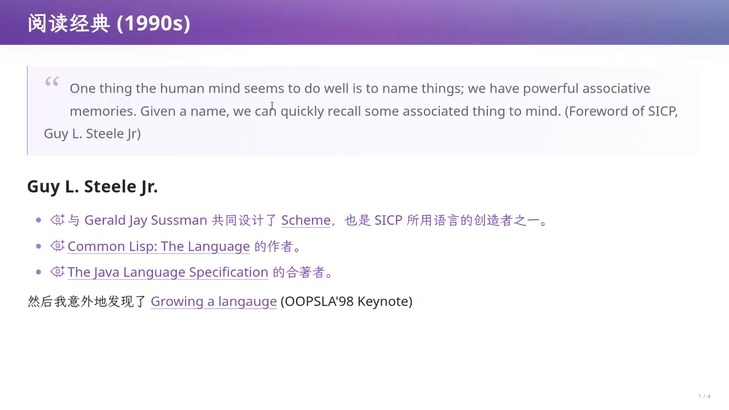
\includegraphics[width=\textwidth]{figures/fig_10_steele_naming.jpg}
\caption{命名、语言与Steele的设计工作\vtag}
\end{figure}
\srcnote{00:34:37--00:34:45}

命名本身还不够。如果同一个名字在几个地方有不同含义，或者名字掩盖了不同的前提，它反而会增加误解。架构中的概念应有稳定的使用条件和组合方式，让名字成为压缩知识的入口。

\subsection{Growing a Language 的设计困境}
讨论推进到 1990 年代的经典时，课堂选择了 1998 年 OOPSLA 的演讲从单音节词开始，遇到更复杂的词汇便当场定义。听众因此经历语言从很小的词汇集合逐步扩展的过程。课堂用这个表演说明，起点极小的语言容易交付，但表达复杂需求很吃力；一次设计一个包办所有需求的大语言，又可能在真正交付前失去机会。

讲者用 Brainfuck 和 C 讨论这个取舍。前者作为极简例子，很难直接阅读；C 易于贴近机器，却在自定义抽象上承担限制。课堂特别提到 \texttt{qsort} 的数组长度、元素大小和比较函数参数：调用者必须自己维持这些参数之间的关系。这里是在讨论表达复杂概念时的成本，不是在否认这些工具能够工作。

\subsection{扩展机制也需要可以组合}
讲者归纳演讲中的方向为：给用户提供创建新概念的工具，而不是不断增加孤立的用途清单。课堂提到泛型、运算符重载、轻量用户自定义类型等扩展能力，也指出某些语言的扩展可能长成难以理解的结构。后者是讲者的设计评价，应与语言具有什么功能区分开。

\begin{importantbox}{可生长性的检查}
不只检查能否再加一个功能，还要检查新功能能否使用既有原语、能否与其他扩展组合，以及是否需要修改公共规则才能工作。扩展可以进入共同结构，才有机会降低未来变化的代价。
\end{importantbox}

上一讲的二维码小语言也可以从这个角度理解：设计者把操作组织成一个中间表示，让不同执行方式复用它。在本讲的语境里，语言设计、模块接口设计与软件架构讨论的是同一类选择：把什么作为稳定的共同表达，把什么交给未来的使用者。

\subsection{从经典建立判断，而不只复制形式}
讲者批评信息洪流中低质量内容对设计品味的影响，鼓励回到经典的实际问题与解决过程。他还把只求通过、无需后续维护的习题代码，与需要长期扩展的软件作了比较。这些是课堂的教学判断，不表示每个练习都没有架构价值。
\begin{figure}[H]
\centering
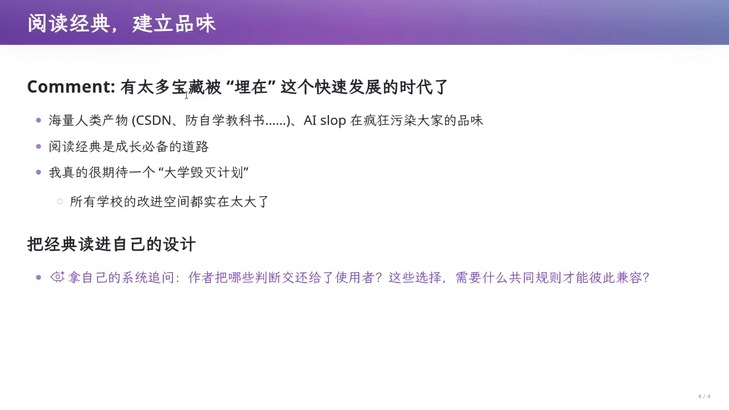
\includegraphics[width=\textwidth]{figures/fig_11_design_taste.jpg}
\caption{从经典中建立可组合设计的判断\vtag}
\end{figure}
\srcnote{00:48:07--00:48:15}

读经典时应把问题带回自己的系统：哪些决定已经固定？什么必须由调用者自行补齐？这种补齐是否有公共规则？如果仍然只有具体功能，没有组合方式，所谓扩展便可能只是在各处新增特殊分支。下一章的 UNIX 展示了共同规则怎样成为可操作的架构。

\subsection{本章小结}
可生长性要求设计一片解空间：当前的核心足够清楚，未来的变化能通过既定规则进入系统。名字帮助压缩知识，扩展机制帮助构造新概念，组合协议则保证这些概念不会变成互不相通的孤岛。

\section{UNIX 为什么能让使用者创造新用途}
\label{sec:unix}
UNIX 的组合能力依靠共同接口。小工具只承担局部任务，使用者却能用 Shell 把它们接成新的流程。课堂认为文本流是关键，因为它让人读输出和程序读输出有机会使用同一种材料。

\subsection{文本流把工具接成流水线}
三条课堂原则可以译为：做好一件事；让程序协作；让程序处理文本流。第三条使前两条有了连接方式。输出可以显示给人、写入文件，也可以成为下一程序的输入。需要调试时，还能截取流水线的中间结果，检查错误来自哪一步。
\begin{figure}[H]
\centering
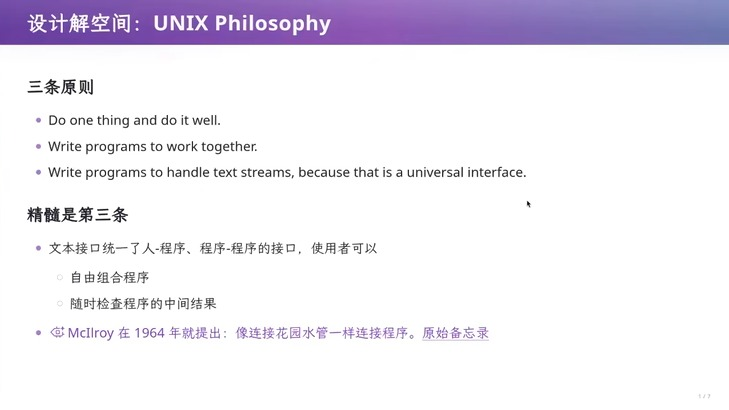
\includegraphics[width=\textwidth]{figures/fig_12_unix_philosophy.jpg}
\caption{UNIX用文本接口连接程序与人\vtag}
\end{figure}
\srcnote{00:49:37--00:49:45}

\begin{importantbox}{接口同时服务执行与观察}
稳定的中间输出既是程序间协议，也是人的观察点。使用者能够单独运行某一步、查看它产生的材料，再决定是否继续组合。这种可检查性是文本接口的重要收益。
\end{importantbox}

课件把 McIlroy 在 1964 年提出的水管式连接思想作为背景。语音转录在约 51:00 给出管道于“1983 年”进入 UNIX 的说法；这个年份与 Bell Labs 的历史说明不符，因此本笔记不采用它作为史实。Bell Labs 资料将实现年份记为 1973 年。这个校注只修正历史时间，不改变课堂关于共同接口的论证。\footnote{补充核查：\href{https://www.nokia.com/bell-labs/research/sdsr/unix-game/}{Bell Labs: The UNIX Game}。}

\subsection{“都是文本”还需要公共约定}
选项、选项参数和操作数要能区分；数据输入、正常输出、诊断输出与退出状态也承担不同职责。标准输入提供数据，标准输出给出结果，标准错误承载诊断，退出状态另行说明执行结果。管道通常连接前一步的标准输出与后一步的标准输入，而不会自动把所有诊断信息当作数据。
\begin{figure}[H]
\centering
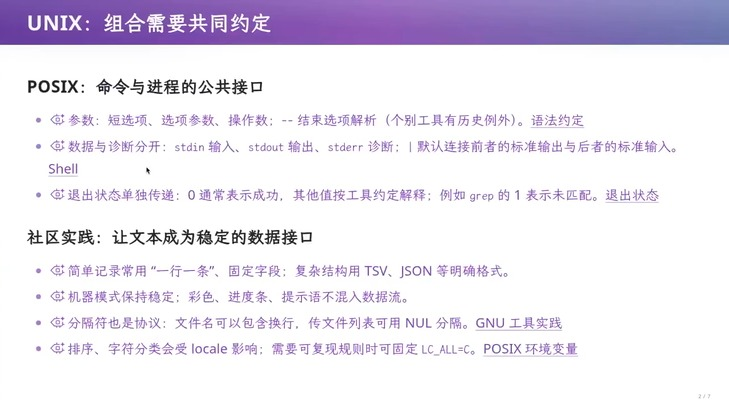
\includegraphics[width=\textwidth]{figures/fig_13_posix_contract.jpg}
\caption{通道退出状态与数据格式的公共约定\vtag}
\end{figure}
\srcnote{00:51:37--00:51:45}

\begin{warningbox}{供机器读取的输出也是协议}
颜色、进度条和“操作成功”提示若混入数据，下一步就可能把它们当成记录。按行处理时还要知道分隔符是否有歧义；文件名允许换行的场景，应使用能够保留边界的约定，例如 NUL 分隔，而不能直接假定一行就是一个文件名。
\end{warningbox}

课堂课件还提示 locale 会影响排序和字符分类。需要可复现的机器处理结果时，应明确环境条件。类似地，退出码 0 通常表示成功，但其他值的含义应查看具体工具约定；例如 \texttt{grep} 的 1 可以表示没有匹配，而不能一概解释成同一种故障。

\subsection{人的判断也可以成为流程中的一步}
\texttt{jq} 从 JSON 中提取字段，\texttt{fzf} 接收候选、让人选择，再输出选择结果。于是书目 JSON、书名提取和人工选择可以形成一条流水线。这里人的判断没有脱离程序接口，而是以输入候选、输出选择的形式加入了组合。
\begin{figure}[H]
\centering
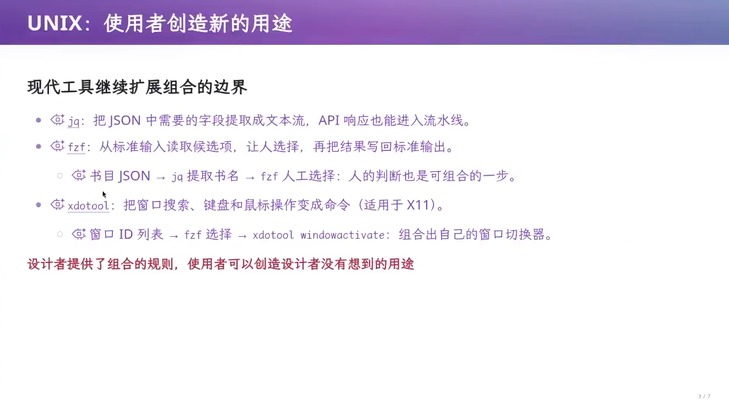
\includegraphics[width=\textwidth]{figures/fig_14_unix_composition.jpg}
\caption{jq fzf xdotool组合出新的用途\vtag}
\end{figure}
\srcnote{00:52:37--00:52:45}

\texttt{xdotool} 将窗口查找、键盘和鼠标操作包装成命令，可在适用的 X11 环境中参与组合。候选窗口 ID 交给选择器，再激活所选窗口，便能构造个人的窗口切换工具。课堂的现场演示则为编辑器组合了一个文件选择菜单：先得到文件候选，再选择，最后交给编辑器打开。
\begin{figure}[H]
\centering
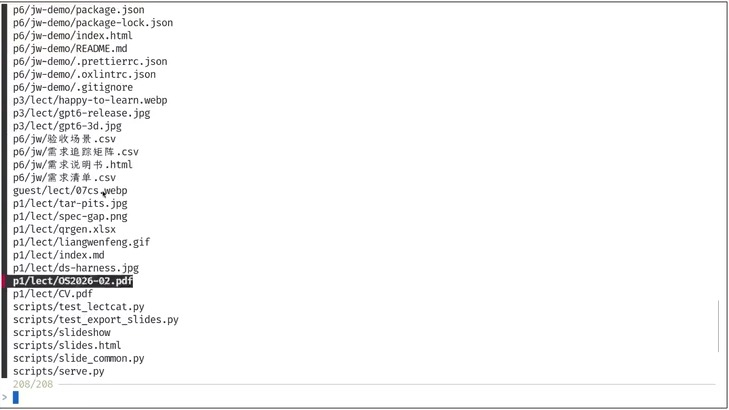
\includegraphics[width=\textwidth]{figures/fig_15_file_picker.jpg}
\caption{课堂演示可组合的文件选择菜单\vtag}
\end{figure}
\srcnote{00:54:07--00:54:15}

\begin{knowledgebox}{哪些能力由谁决定}
工具作者确定输入输出和局部操作的语义；使用者决定如何连接它们。设计者无需列出所有书目管理、文件打开或窗口切换场景，就能支持这些场景。共同规则扩大用途，但不会替使用者证明任意组合都正确。
\end{knowledgebox}

\subsection{本章小结}
UNIX 用文本、通道、格式与执行结果的约定，把局部工具变成可组合材料。架构的价值体现在它允许后来者创造新的流程。数据库与 Internet 也采取了类似方向，只是它们选择了不同的稳定抽象与变化边界。

\section{数据库与网络怎样把变化隔离在不同层}
\label{sec:systems}
通用系统的共同任务，是提供足够稳定的抽象，让应用不必每次从底层重新开始。关系数据库分开逻辑关系与物理存储，Internet 分开上层用途与通信基础。理解这个分离，才能看清它们怎样承受跨越几十年的变化。

\subsection{关系模型让查询不绑死于存储}
课堂引用 Codd 在 1970 年提出的关系模型，其目标包括让用户不必随数据表示、规模和访问变化而重写数据使用方式。逻辑层说明有哪些实体和关系，物理层决定记录怎样组织、使用哪些索引，以及查询怎样执行。二者分开，才能分别演化。
\begin{figure}[H]
\centering
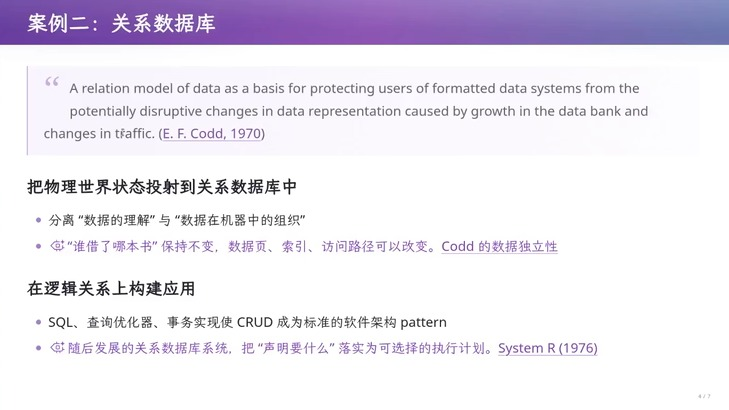
\includegraphics[width=\textwidth]{figures/fig_16_relational_model.jpg}
\caption{逻辑关系与物理表示的分离\vtag}
\end{figure}
\srcnote{00:56:07--00:56:15}

图书馆的例子把这种分离画得很直观。读者、图书和借阅关系表达谁借走了哪本书；查询既可以从读者出发，也可以从馆藏出发。堆文件与索引、分区与索引是存储选择，不应改变同一笔借阅在逻辑上的含义。
\begin{figure}[H]
\centering
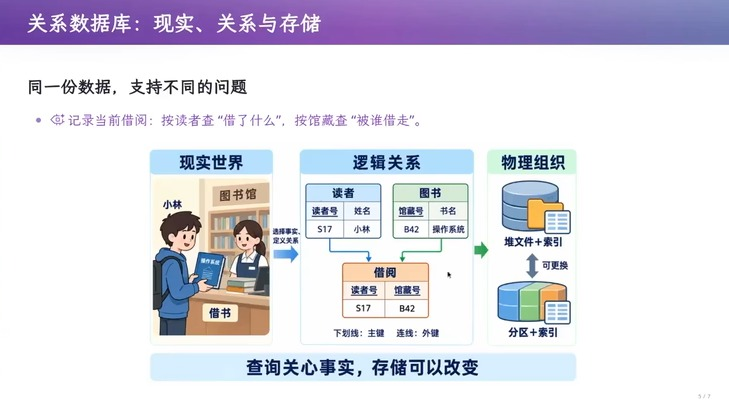
\includegraphics[width=\textwidth]{figures/fig_17_library_relationships.jpg}
\caption{读者图书借阅关系与存储布局\vtag}
\end{figure}
\srcnote{00:58:07--00:58:15}

\begin{importantbox}{应用依赖逻辑含义，底层优化执行方式}
需要什么结果与怎样读取数据，可以交给不同层处理。接口稳定并不意味着底层不会影响性能，而是表示应用不应因为某次物理布局调整就被迫改变业务含义。
\end{importantbox}

\subsection{查询、优化与事务共同支撑业务操作}
SQL 提供表达查询的语言，优化器选择执行方案，事务把应共同完成的读写组织起来。创建、读取、更新和删除，即 CRUD，成为许多信息系统的共同骨架。课件还把 1976 年的 System R 放在这个发展脉络中，用来说明声明结果与选择执行方案的分工。

这些机制没有预先列出全部教务查询、图书馆报表和商城需求。数据库给出关系、约束和操作规则，由使用者决定模式与查询。因此，数据库本身也在提供解空间。课堂对其扩展能力的强调，是为了说明抽象的价值，不能据此推断任意查询都能无限扩展或没有运行成本。

\subsection{网络把应用需求放在共同传输基础之上}
手机通过 TCP 访问 HTTPS 服务时，应用表达请求，传输与安全机制处理相应职责，IP 组织跨网络传送，链路层处理相邻设备间的数据移动。图中手机侧的 Wi-Fi 和服务器侧的以太网可以不同，业务请求却不必逐段理解这些硬件细节。
\begin{figure}[H]
\centering
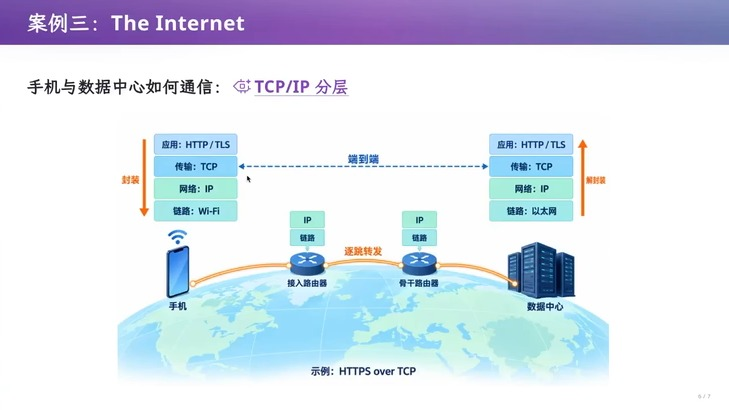
\includegraphics[width=\textwidth]{figures/fig_18_tcp_ip_layers.jpg}
\caption{手机到数据中心的分层传输\vtag}
\end{figure}
\srcnote{00:59:07--00:59:15}

TCP 提供可靠传输的抽象，同时也要处理拥塞、连接管理与中断等具体问题。它把一部分复杂性集中到传输层，让应用不用各自重新实现同一套机制；这不表示网络中断、服务失效和应用错误因此不存在。

\subsection{变化中的局部替换与整体延续}
课堂引用 1996 年 6 月的 RFC 1958，强调技术变化是架构必须承受的条件。远程登录从 Telnet 转向 SSH，许多文件与信息访问用途迁向 HTTPS，SMTP 与 IMAP 等协议仍承担邮件功能。上层应用改变，底层共同协作规则仍能继续提供基础。
\begin{figure}[H]
\centering
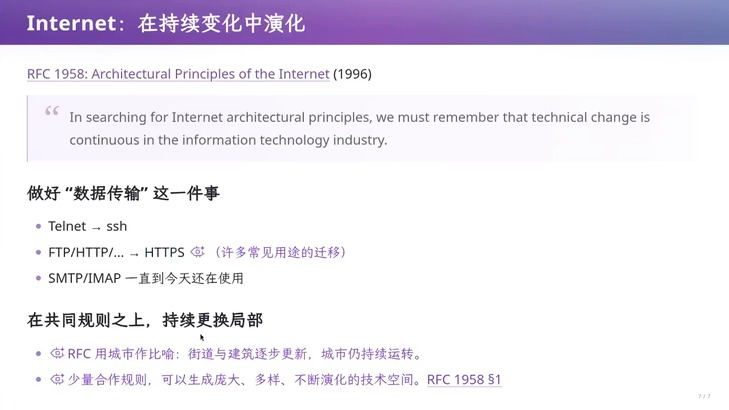
\includegraphics[width=\textwidth]{figures/fig_19_internet_evolution.jpg}
\caption{网络基础与应用的独立演化\vtag}
\end{figure}
\srcnote{01:02:37--01:02:45}

城市的类比帮助解释这种延续：街道和建筑可以改建，城市仍继续运转。网络也不必在每次新应用出现时整体推倒重来。在共同规则上更换局部，是可生长架构的一种表现，而不是架构永远不变的证明。

\subsection{通用抽象层怎样承载技术浪潮}
课件从 1964 年 IBM System/360、1969 年 UNIX、1970s 的 Smalltalk，列到 1989--1991 年的 Web、2008 年 Android 和 2014 年 Kubernetes，比较它们为通用应用提供的抽象。这个时间轴用于课堂的架构比较，不表示各系统在同一条件下出现或遵循完全相同的技术机制。
\begin{figure}[H]
\centering
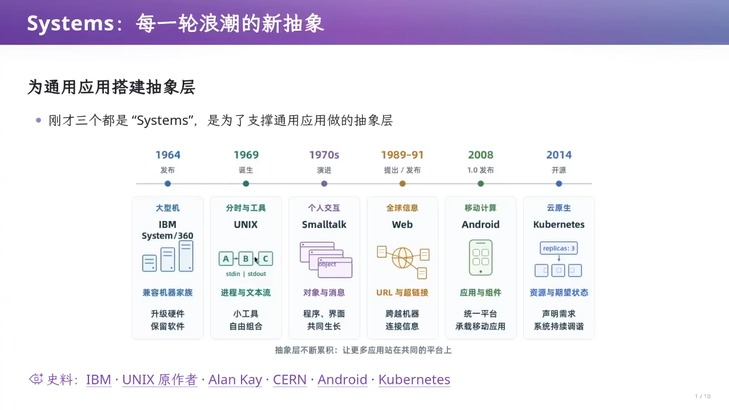
\includegraphics[width=\textwidth]{figures/fig_20_systems_waves.jpg}
\caption{通用系统的抽象层与技术浪潮\vtag}
\end{figure}
\srcnote{01:04:07--01:04:15}

它们分别隐藏机器差异、连接进程、组织对象、连接资源、封装应用服务或管理集群状态。共同之处在于让上层用更接近目标的概念工作。具体客户的软件已有这些地基，接下来仍要决定自身业务规则和界面如何组织。

\subsection{本章小结}
关系模型稳定数据的逻辑解释，通信协议稳定协作的层次边界。双方都让应用与底层获得一定的独立演化能力。地基提供了通用能力，但客户的软件仍会因重复业务规则、展示耦合和状态管理方式而增加复杂性。

\section{MVC 怎样让不同变化各有归属}
\label{sec:mvc}
一个信息系统最直接的组织方式，是把每次页面操作对应为数据库读写，再把查询结果显示出来。这个方式能很快做出功能，但业务规则若散落在各页面中，修改时就需要逐一寻找。MVC 用职责分离来控制这种变化传播。

\subsection{页面与事务为什么容易长在一起}
课堂请读者想象回到 1998 年或 2000 年：操作系统、数据库和网络已经提供基础能力，页面发出请求，服务端执行事务，再返回 HTML。学生选课就是读取课程、检查条件、记录选择和返回结果的一个流程。容量限制却也可能被复制到普通选课、管理员补选和导入页面中。
\begin{figure}[H]
\centering
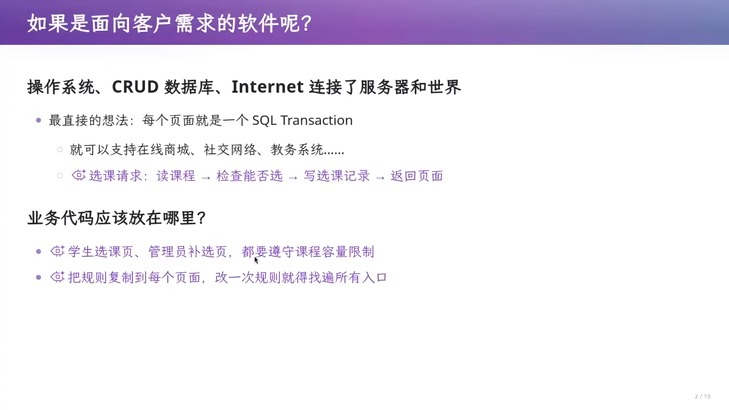
\includegraphics[width=\textwidth]{figures/fig_21_page_transaction.jpg}
\caption{页面事务模式与规则重复\vtag}
\end{figure}
\srcnote{01:05:37--01:05:45}

页面可以工作，规则仍可能不一致。一处修改课程容量的解释后，如果另一入口没有同步更新，两份代码便开始代表不同业务。问题来自同一个决定被重复实现，单纯把页面写得更整齐无法消除它。

\subsection{模板改善页面表达，不自动分离业务}
课堂回顾 Java Web 浪潮及自动内存管理对开发方式的影响。与在程序里逐行拼接 HTML 相比，模板让 HTML 保持页面形状，在指定位置填入数据或执行展示循环。课堂也用拼接提示词与 Jinja2 模板作类比：把变量放进明确的槽位，比长期维护字符串相加的表达式更容易理解。
\begin{figure}[H]
\centering
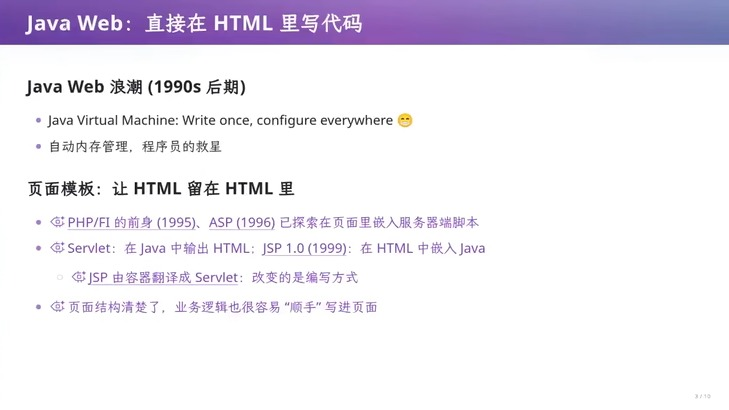
\includegraphics[width=\textwidth]{figures/fig_22_java_templates.jpg}
\caption{HTML模板与服务端代码的关系\vtag}
\end{figure}
\srcnote{01:07:07--01:07:15}

课件列出 PHP（1995）、ASP（1996）、JSP 1.0（1999），再到 JSTL 1.0（2002）与 JSP 2.0（2003）。这个演进说明写法怎样从脚本片段延伸到表达式与标签。JSP 容器把页面翻译为 Servlet，改变的是作者描述页面的方式。
\begin{figure}[H]
\centering
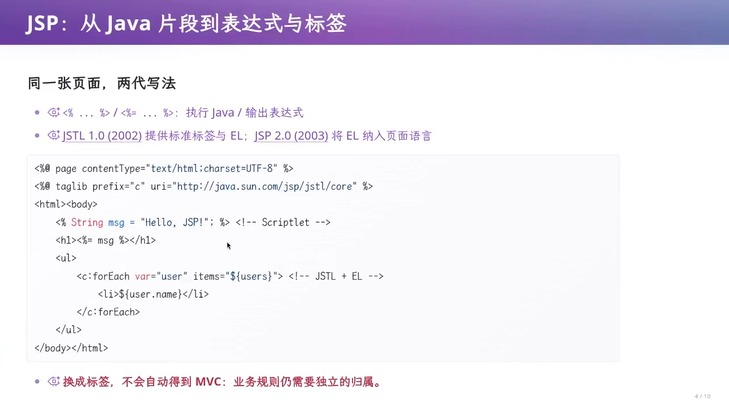
\includegraphics[width=\textwidth]{figures/fig_23_jsp_syntax.jpg}
\caption{JSP脚本表达式与标签的展示机制\vtag}
\end{figure}
\srcnote{01:10:07--01:10:15}

\begin{warningbox}{模板语法与业务边界是两个决定}
用标签代替脚本，可以改善显示循环的表达；若容量判断、权限判断和业务写入仍埋在各页面里，职责混杂就仍然存在。业务规则需要明确归属，不能期待语法替换替自己完成架构设计。
\end{warningbox}

\subsection{Model、View 与 Controller 的具体职责}
MVC 的早期材料发表于 1979 年，最初讨论交互式界面；课堂再把它用于 Web 业务。Model 封装数据、状态和业务规则，View 展示结果，Controller 接收输入并协调操作。Model 不是数据库表的同义词，课程容量和冲突检查也属于它应表达的业务含义。
\begin{figure}[H]
\centering
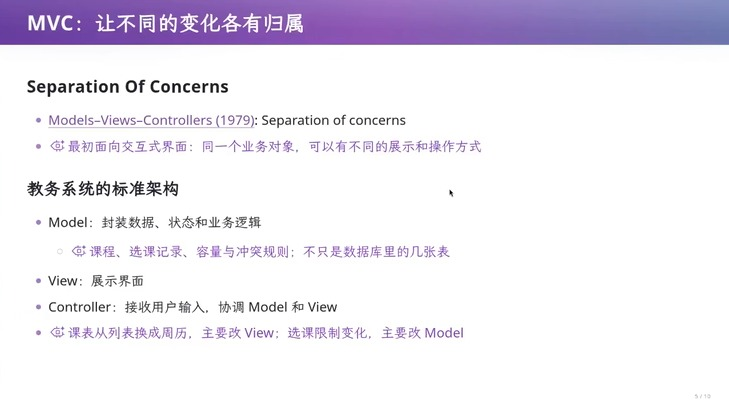
\includegraphics[width=\textwidth]{figures/fig_24_mvc_roles.jpg}
\caption{MVC中的业务规则展示和输入职责\vtag}
\end{figure}
\srcnote{01:12:37--01:12:45}

\begin{center}
\begin{tabular}{p{2cm}p{5.2cm}p{6.2cm}}
\toprule
角色 & 负责的知识或操作 & 选课系统中的例子\\
\midrule
Model & 业务数据、状态、规则 & 课程、选课记录、容量与先修检查\\
View & 呈现业务结果 & 课表、成功信息、失败原因\\
Controller & 接收请求并协调处理 & 解析选课输入、调用规则、选择展示\\
\bottomrule
\end{tabular}
\end{center}

选课请求进入 Controller，由 Model 检查资格、时间和容量，并在适当的事务边界内完成记录，View 再呈现结果。图中还标出请求、参数、业务处理、事务与模板数据的路径。职责之间通过具体信息协作，而不是各自包含一份完整业务实现。
\begin{figure}[H]
\centering
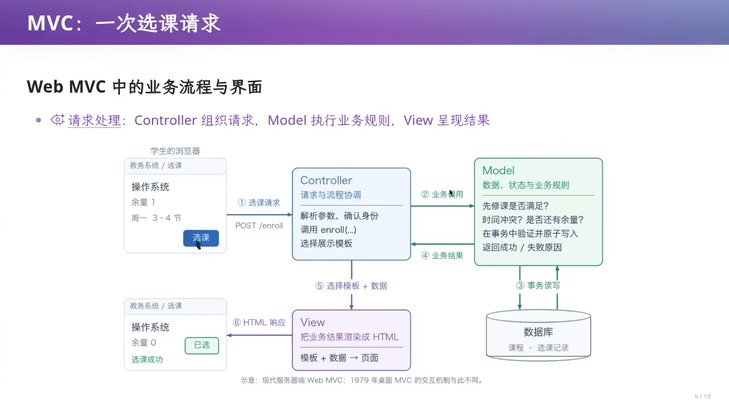
\includegraphics[width=\textwidth]{figures/fig_25_mvc_enrollment.jpg}
\caption{一次选课请求经过MVC的路径\vtag}
\end{figure}
\srcnote{01:13:07--01:13:15}

\begin{importantbox}{先辨认变化属于谁}
课表从列表改成周历，主要改变展示；选课条件变化，主要改变业务规则；新增管理员入口，需要明确权限并复用适用规则。职责分离的收益，是同一种变化有可以追踪的归属。
\end{importantbox}

\subsection{本章小结}
MVC 为业务知识、界面展示和输入处理建立边界，模板为展示提供表达工具。它能减少规则在多个页面中的重复，却还没有回答一个现代界面的普遍问题：搜索词、展开菜单和悬停状态既不属于业务数据库，又确实会改变显示结果。

\section{界面状态怎样成为可计算的依赖}
\label{sec:ui}
界面自身也有需要管理的状态。同一份课程数据，配上不同筛选词，应该显示不同列表。把这些状态和它们的依赖明确表达出来，框架才有机会维护更新，开发者也不必在每个事件中记住所有需要修改的控件。

\subsection{持久化与建模是两件事}
菜单是否展开、鼠标悬停在哪里、查询词是什么，通常不会存进业务数据库，但都参与决定当前界面。课件将这一点表示为：
\[
  \mathrm{View}=\operatorname{render}(\mathrm{Model},\mathrm{ViewState}).
\]
\begin{itemize}
\item \(\mathrm{Model}\)：界面所使用的业务数据及其含义。
\item \(\mathrm{ViewState}\)：筛选词、选择或展开状态等展示相关输入。
\item \(\operatorname{render}\)：根据这些输入描述界面的过程。
\item \(\mathrm{View}\)：当前应该呈现的界面。
\end{itemize}
\begin{figure}[H]
\centering
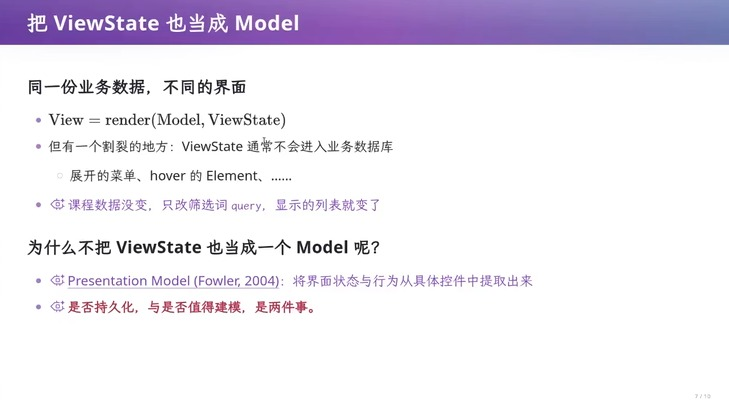
\includegraphics[width=\textwidth]{figures/fig_26_view_state.jpg}
\caption{界面状态独立于业务持久化\vtag}
\end{figure}
\srcnote{01:14:07--01:14:15}

\begin{knowledgebox}{暂时存在的状态也值得认真组织}
不需要持久保存，并不等于不需要建模。若展示信息分散藏在控件和事件回调中，开发者就必须手工追踪它们之间的同步关系。将状态明确表示，才能讨论它依赖什么以及怎样更新。
\end{knowledgebox}

\subsection{React：用一次渲染的状态描述界面}
React 的课堂模型是组件依据属性和状态描述当前界面，用户事件通过状态更新入口请求下一次渲染。\texttt{query} 决定筛选词，课程数据和筛选词共同决定可见列表；已有输入能够计算出的列表，不必再作为一份可独立修改的状态保存。
\begin{figure}[H]
\centering
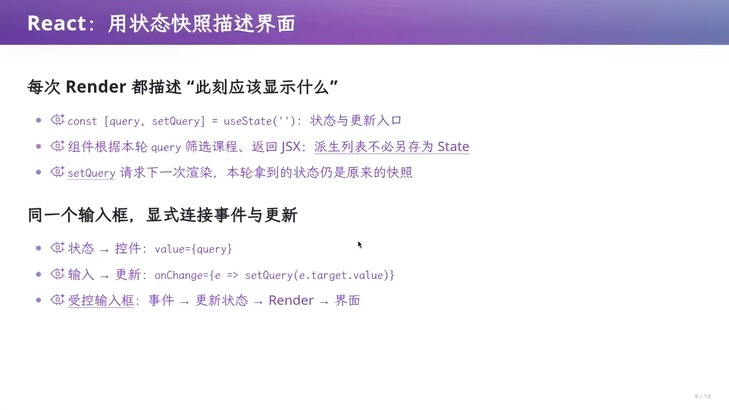
\includegraphics[width=\textwidth]{figures/fig_27_react_snapshot.jpg}
\caption{React用状态快照描述界面\vtag}
\end{figure}
\srcnote{01:15:37--01:15:45}

以下是按课件机制整理的最小代码片段，省略组件外壳与课程列表的具体展示，保留状态、派生结果、输入值和事件更新之间的关系：
\begin{lstlisting}[language=Java,caption={React 课程筛选：保存必要状态，计算派生列表}]
const [query, setQuery] = useState('');
const visibleCourses = courses.filter(
  course => course.name.includes(query)
);
return <input
  value={query}
  onChange={e => setQuery(e.target.value)}
/>;
\end{lstlisting}

\texttt{setQuery} 请求更新，并不会立即改写当前这次渲染已经拿到的状态变量。下一次渲染使用新的快照。课堂还指出，如果界面有很多元素，框架需要处理更新工作的成本；开发者声明状态到界面的关系，框架承担渲染与更新组织的一部分复杂性。这个教学模型不等于保证每次输入只更新某一个固定 DOM 节点。

\subsection{Vue：声明响应式状态与双向连接}
Vue 的课堂模型用响应式状态保存 \texttt{query}，用 \texttt{computed} 表达可见课程由哪些输入计算出来。\texttt{v-model} 包装输入框的两条关系：状态决定控件显示值，输入事件反过来更新状态。绑定关系写出来后，由框架追踪相应变化。
\begin{figure}[H]
\centering
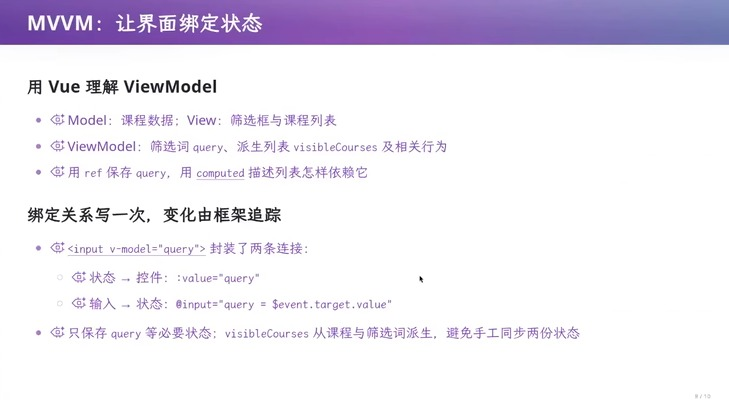
\includegraphics[width=\textwidth]{figures/fig_28_vue_binding.jpg}
\caption{Vue声明状态与输入的绑定\vtag}
\end{figure}
\srcnote{01:17:37--01:17:45}

\begin{lstlisting}[caption={Vue 课程筛选：按课件机制整理的表达片段}]
const query = ref('');
const visibleCourses = computed(() =>
  courses.value.filter(c => c.name.includes(query.value))
);
// template:
// <input v-model="query" />
\end{lstlisting}

片段中的 \texttt{courses.value} 假定课程数据也采用相应响应式表示，完整应用仍需要提供课程数据与模板列表。这里展示的是依赖关系，不能脱离这些输入独立运行。

\subsection{比较更新方式，避免重复保存派生状态}
Vue 通过绑定语法与依赖追踪表达更新，React 在事件中显式调用状态更新入口。两种写法都试图让界面从状态派生。课件同时限定，输入框上的双向绑定不等于整个组件系统任意双向流动，父到子的属性仍有自己的传递方向。
\begin{figure}[H]
\centering
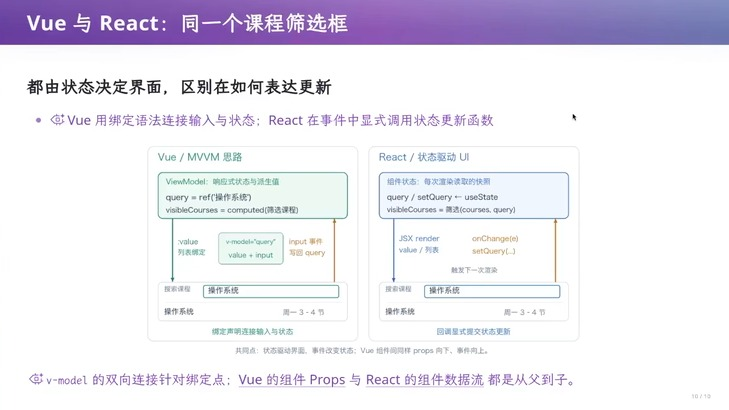
\includegraphics[width=\textwidth]{figures/fig_29_vue_react_comparison.jpg}
\caption{课程筛选框的两种更新模型\vtag}
\end{figure}
\srcnote{01:18:37--01:18:45}

\begin{center}
\begin{tabular}{p{3cm}p{5.1cm}p{5.3cm}}
\toprule
问题 & Vue 的课堂表达 & React 的课堂表达\\
\midrule
筛选词 & \texttt{ref} 中的 \texttt{query} & \texttt{useState} 的状态快照\\
可见列表 & \texttt{computed} 描述依赖 & 渲染时按输入计算\\
输入更新 & \texttt{v-model} 连接值与事件 & \texttt{value} 加 \texttt{onChange}\\
共同原则 & \multicolumn{2}{p{10.4cm}}{保存必要状态，让其他结果沿已表达的关系派生}\\
\bottomrule
\end{tabular}
\end{center}

\begin{warningbox}{同一结果不要有多个独立写入源}
如果可见课程已经由课程数据与筛选词确定，却另存一份可以随意修改的列表，就新增了同步责任。输入变了、列表没改，便产生两个互相矛盾的界面状态。需要缓存时，也应保留它的来源与失效条件。
\end{warningbox}

\subsection{本章小结}
界面框架把展示相关的状态和计算依赖摆到明面上，使输入、更新与派生结果更容易理解。讲者偏好 React 的表达，但把两种模型都放在隔离复杂性的框架中讨论。相同原则进入长业务流程后，还要面对过去事实、当前结果与未来预期之间的关系。

\section{记账案例怎样把凭证编译为状态变化}
\label{sec:ledger}
把复杂代码放进 Model，不能自动解决本质复杂性。订单会经历下单、锁库存、优惠、支付、风控、发货、退款和对账，后面的失败可能影响前面的决定。记账案例提供另一种组织思路：保留原始业务材料，把它翻译为含义确定的动作，再由程序计算报表。

\subsection{一个 status 字段承担不了全部历史}
当前状态可以用表和字段保存，但一个状态值常常同时暗示过去已经做过什么、现在等待什么、未来还应完成什么。某一步被人工特批覆盖后，若只改结果而未保存依据，就可能出现风控失败却进入下一环节，或者学生同时满足与不满足某些毕业条件的矛盾。
\begin{figure}[H]
\centering
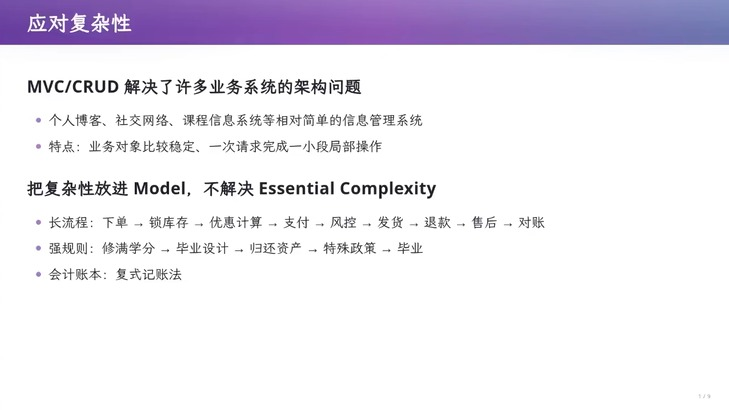
\includegraphics[width=\textwidth]{figures/fig_30_long_workflow.jpg}
\caption{MVC不能消除长流程的领域复杂性\vtag}
\end{figure}
\srcnote{01:20:07--01:20:15}

讲者用这些情况说明长流程为何难以维护。即使最终没有阻止业务完成，系统内部失去解释依据仍是问题。这里对教务系统中不一致数据的描述来自他的观察和判断，本笔记不把它扩展为对具体数据库内容的独立审计结论。

\subsection{复式记账提供可检查的关系}
复式记账要求一笔业务通过相互对应的账户记录，借方与贷方金额合计相等。用课堂所讨论的试算平衡，可以写成：
\[
  \sum_i D_i=\sum_j C_j.
\]
\begin{itemize}
\item \(D_i\)：同一笔业务中第 \(i\) 项借方记录的金额。
\item \(C_j\)：同一笔业务中第 \(j\) 项贷方记录的金额。
\item 两个求和分别汇总该笔业务的借方和贷方记录。
\end{itemize}

借与贷在这里是记账方向，不能直接套用日常语言中的借入、借出。约束给程序提供了一种发现不一致的机会，却不能证明记录符合真实业务。金额相等的错误分类或重复记录，也可能通过平衡检查。

\begin{warningbox}{约束成立不代表业务真实}
试算平衡只能检查它表达的关系。原始凭证是否被理解正确、账目类别是否合适、同一业务是否重复输入，仍然要核对。课堂中的模型生成方案是架构实验，不是经审计认证的会计软件。
\end{warningbox}

\subsection{语言模型作前端，账本程序决定动作语义}
案例把流程分为原始凭证、记账动作、状态变化。语言模型理解人的材料，将它翻译成系统支持的操作，例如课件上的 \texttt{CNY(75)} 金额与财务费用动作；程序再按共同规则更新有关报表。它不像让模型逐格填写最终表格，因为同一动作的多个后果由一次确定的解释产生。
\begin{figure}[H]
\centering
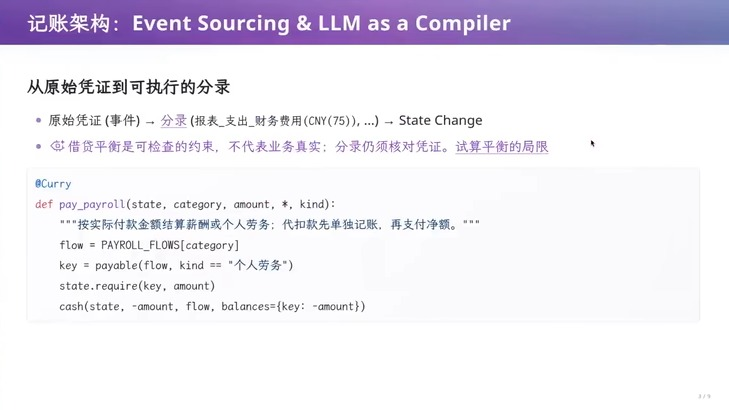
\includegraphics[width=\textwidth]{figures/fig_31_ledger_compiler.jpg}
\caption{原始凭证到受约束记账动作\vtag}
\end{figure}
\srcnote{01:24:37--01:24:45}

\begin{importantbox}{编译器式分工}
模型负责把材料翻译成受约束的表示，程序负责这份表示的执行含义。动作是否符合凭证需要审查，动作执行是否保持约束则可以另行检查。把两个问题分开，比把所有报表数值交给一次自由生成更容易追溯错误。
\end{importantbox}

课堂展示的工资结算片段如下。它依赖项目中的金额类型、分类表及状态操作，不能单独运行；中文业务类别保留课件含义：
\begin{lstlisting}[language=Python,caption={课件工资结算操作：检查应付款，再同步减少现金与应付余额}]
@Curry
def pay_payroll(state, category, amount, *, kind):
    flow = PAYROLL_FLOWS[category]
    key = payable(flow, kind == "个人劳务")
    state.require(key, amount)
    cash(state, -amount, flow, balances={key: -amount})
\end{lstlisting}

函数先依据类别确定现金流分类和对应应付款项，再检查可结算余额，同时减少现金与应付余额。课件说明代扣款应先单独记账，再支付净额。因此确认费用、形成应付与实际支付应被区分；付钱时若重新确认同一费用，就会造成重复记录。\texttt{@Curry} 的用法则把确定下来的部分参数绑定起来，减少后续动作表达的重复。

\subsection{同一动作怎样共同影响不同报表}
课堂的规则表将记账动作映射到资产负债表、利润表及现金流量表。屏幕中 \(+1.00\) 与 \(-1.00\) 表示单位动作对各项目的影响方向，用来说明联动规则，并不是企业真实金额。表中的现金、负债、利润和权益，应来自同一动作语义，而不是分别手工补数。
\begin{figure}[H]
\centering
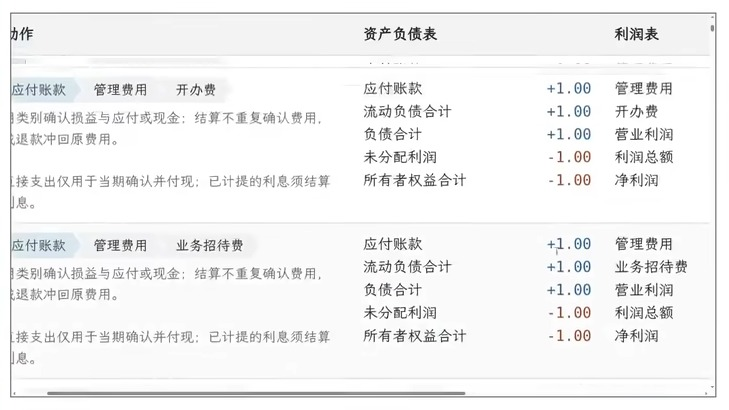
\includegraphics[width=\textwidth]{figures/fig_32_ledger_rules.jpg}
\caption{记账动作共同影响多个报表项目\vtag}
\end{figure}
\srcnote{01:27:07--01:27:15}

\newpage
具体银行收支例子包含财务费用支出 75 元和利息收入 22.07 元。报表中的货币资金净变化由同一组动作得到：
\[
  \Delta M=22.07-75=-52.93\quad\text{元}.
\]
\begin{itemize}
\item \(M\)：这个例子中的货币资金项目。
\item \(\Delta M\)：这两笔动作造成的净变化。
\item 22.07 元为示例利息收入，75 元为示例财务费用支出。
\end{itemize}
\begin{figure}[H]
\centering
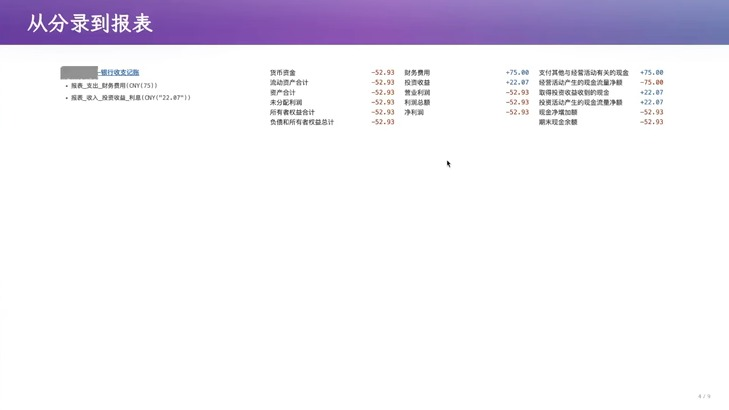
\includegraphics[width=\textwidth]{figures/fig_33_ledger_results.jpg}
\caption{75元费用与22.07元收入的报表结果\vtag}
\end{figure}
\srcnote{01:29:37--01:29:45}

图中多个合计项目出现 \(-52.93\)，反映同一组动作沿工具规则产生的结果。阅读者应同时查原始动作和项目分类，不能因为很多格相同就认定所有会计处理都正确。课堂还用今天收 1,000 元、之后再减少 1,000 元的口头例子，说明记录过程可以保留当前净额无法说明的来由。

\subsection{本章小结}
记账架构把凭证理解、动作表达和报表计算分开。它保留可审查的输入，并让多个派生数值共享一套规则。真正困难的问题仍在：事实如何记录、解释何时变更，以及过去的过程怎样决定今天的结果。

\section{事件溯源怎样把一致性问题变成计算问题}
\label{sec:events}
事件溯源的关键，是保存已经发生的事实，再计算需要的当前视图。它不会消除领域约束，但能把事实、解释与预期分开，使当前结果有一条可以重放和查证的来源路径。

\subsection{过去、现在与未来不要挤在一个状态里}
合同已经签订，是过去的事实；正在等待付款，是当前流程情况；将来是否交货、是否发生坏账，则包含预期。若一个可变状态同时承担三者，修改结果时就容易丢失它从哪里来、为什么改变的线索。
\begin{figure}[H]
\centering
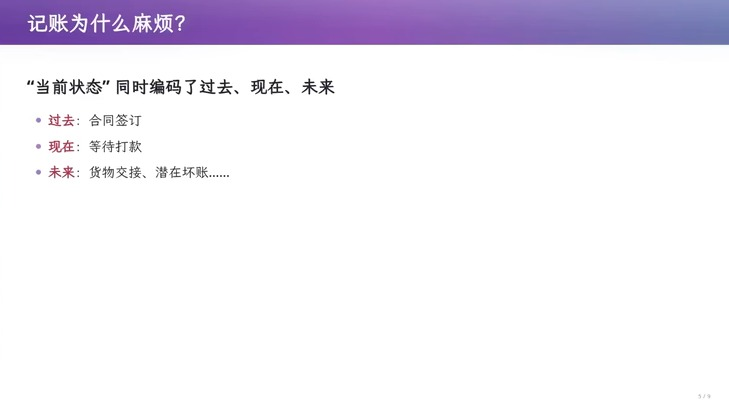
\includegraphics[width=\textwidth]{figures/fig_34_past_present_future.jpg}
\caption{当前状态揉合过去现在与未来\vtag}
\end{figure}
\srcnote{01:31:37--01:31:45}

事件溯源把过去保存为事实，把现在看作事实经规则处理后的视图，把未来当作尚未兑现的预期。情况没有按预期发展，就追加新的事实；先前有错误，也应以可解释的更正、冲销或修正记录处理，而不是偷偷抹掉历史。
\begin{figure}[H]
\centering
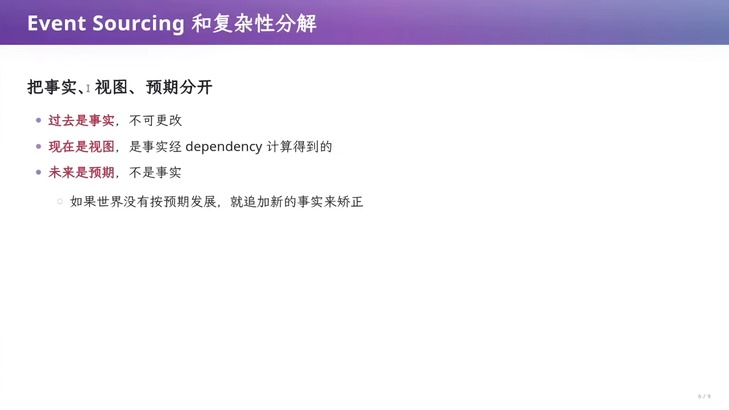
\includegraphics[width=\textwidth]{figures/fig_35_event_sourcing.jpg}
\caption{事件事实计算视图和预期的分离\vtag}
\end{figure}
\srcnote{01:34:07--01:34:15}

\begin{importantbox}{记录变化的来由，才能重新解释结果}
现在不是无来由的字段集合。付款完成、费用确认、成绩更正与经过批准的特例，均应留下足以解释后续计算的材料。不可变历史指避免用隐蔽覆盖伪装过去，并不表示系统永远不能纠正错误。
\end{importantbox}

\subsection{成绩变化怎样传播到毕业判断}
课堂回到教务系统：课程成绩决定已通过课程集合，通过课程和适用培养方案决定学分，再影响准出或毕业相关判断。若这些结果被当作分别写入的独立事实，更正一门课时就必须记住所有后续字段；遗漏一个，当前状态就会不一致。
\begin{figure}[H]
\centering
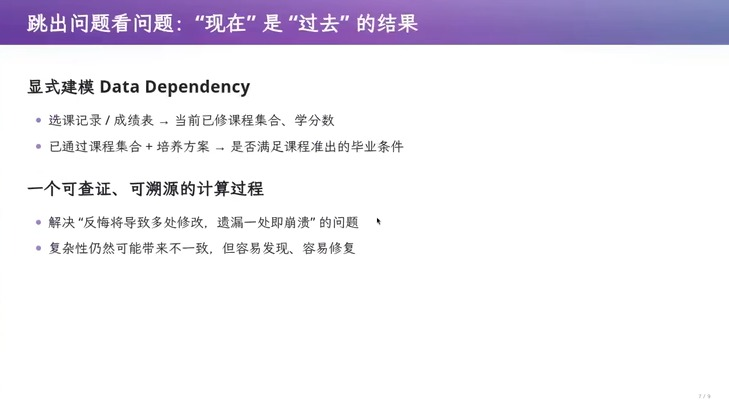
\includegraphics[width=\textwidth]{figures/fig_36_education_dependencies.jpg}
\caption{成绩课程学分毕业结论的依赖\vtag}
\end{figure}
\srcnote{01:36:37--01:36:45}

课堂用计算机系统基础课从通过变为不通过的情境，说明先修资格、学分与后续选课都可能受影响。讲者还举复核后扣回 20 分的假设故事；它是帮助理解变化传播的例子，不能被理解为实际发生的个案记录。

把依赖显式表达后，可以重新处理事实与计算，确定哪些结果改变。系统并不会替学校决定已选上的后续课程应怎样处置；这仍是需要明确的业务规则。架构的改进在于这些问题有共同的数据依据与计算路径，不再靠无来源地修改某个毕业标志隐藏矛盾。

\subsection{特批和规则版本也必须有位置}
如果经授权认为某个学生可以毕业，应记录批准对象、范围和依据，使计算能解释为什么通过。直接将结果改为 1，会使下一次重新计算不知道如何重现这次决定。课程准出条件也不能代表毕业设计、资产归还等所有其他要求。

重现历史结果还需要当时适用的输入。计算机系统基础课的学分可能变动，不同年份培养方案也可能不同。重新计算时不能把今天的学分或汇率悄悄代入过去。记录事实之外，还要保存或能解析相应规则与外部输入的版本。

\begin{warningbox}{重建内部状态不应重复外部动作}
重放可以重新计算现金余额，却不能再次发送已经完成的付款。对外部世界的动作，与内部状态重建必须有清楚边界。保存历史只提供重算材料，不会自动解决外部副作用、输入版本和错误规则的问题。
\end{warningbox}

\subsection{从事实计算视图，也能做条件推演}
讲者进一步指出，已有历史与计算过程可以成为未来情境推演的基础。例如在当前订单处于支付环节时，分别追加风控成功或失败的假设，观察后续状态；在账本中，假设部分应收款无法收回，观察可能的影响。

这是架构提供的能力，不是预测已经可信的证明。课堂明确把风险评估建立在额外模型与假设之上。假设没有发生，便不应混进正式事实历史；推演结果也不应冒充实际报表或业务结论。

\subsection{讲者对 SQL 的批评应怎样理解}
讲者借用“Billion Dollar Mistake”这个说法，批评任意计算关系没有充分成为可直接表达与管理的一等公民。他针对的是数据库、应用代码及其他状态之间的计算依赖，不是说 SQL 不会查询、没有视图，或关系数据库完全不能表达约束。
\begin{figure}[H]
\centering
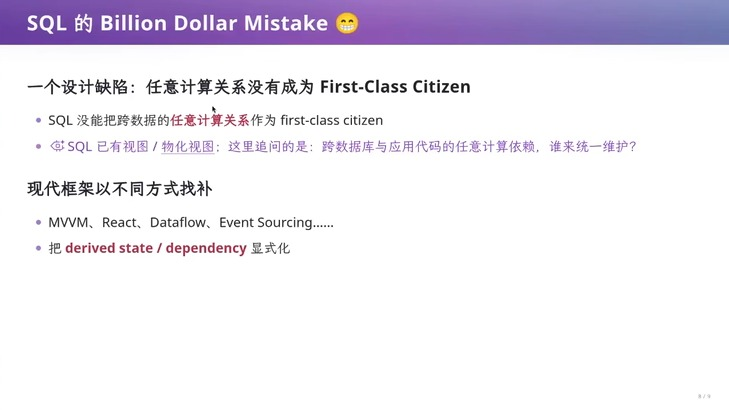
\includegraphics[width=\textwidth]{figures/fig_37_sql_dependency_critique.jpg}
\caption{讲者对跨层计算依赖的批评\vtag}
\end{figure}
\srcnote{01:38:07--01:38:15}

一个查询结果、缓存字段或毕业标志，可能依赖复杂业务逻辑。基础数据变化后，谁判断它失效，谁重算，又怎样找到原始依据？若这些关系只是散落在代码中的约定，即便事务内部一致，系统跨层也仍可能留下矛盾。课堂把 MVVM、React、Dataflow 与 Event Sourcing 放在一起，作为让派生状态与依赖显式化的不同思路；它们并不因此成为同一种技术，也不能据此断言它们有相同历史起因。

\subsection{本章小结}
事件溯源保留事实，让当前状态沿规则计算出来。复杂性从多处状态必须同步，转向输入与计算是否正确。计算仍会错，派生结果也可能暂时滞后，但留下了重跑、测试、审计和依赖分析的材料。架构由此为变化与修正建立了可追溯的边界。

\section{总结与延伸}
\label{sec:summary}
本讲最后的落点，是尽可能保存足以重建其他信息的真实来源，让其余状态成为计算的结果。这样可以把许多状态一致性问题，转化为可以定位、测试和重算的计算正确性问题。这里的“真实来源”不是某个听起来可靠的文件名，而是能够说明事实、适用规则及外部输入的一组材料。
\begin{figure}[H]
\centering
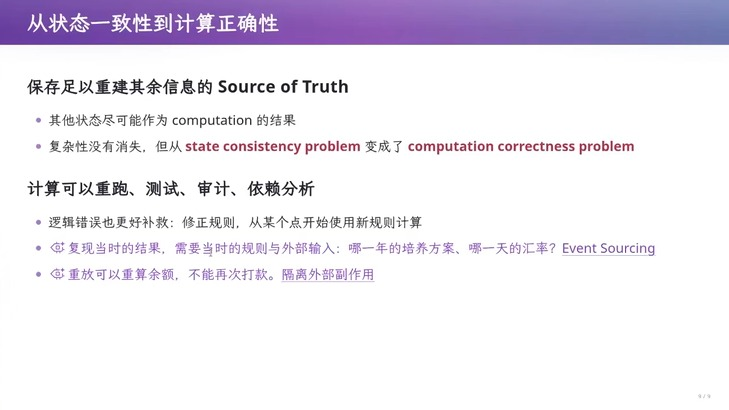
\includegraphics[width=\textwidth]{figures/fig_38_computation_correctness.jpg}
\caption{保存事实并重算可检查的派生状态\vtag}
\end{figure}
\srcnote{01:39:37--01:39:41}

\subsection{把几个案例连成一个判断方法}
本笔记将课堂论证归纳为一条检查路径。先识别不能消除的领域约束，再把它们分解成能单独理解的概念；然后确定共同接口，让新增用途可以组合；最后明确哪些是输入事实、哪些是派生结果，以及修改输入后怎样得到新结果。

UNIX 通过文本与通道安排组合，数据库通过逻辑关系屏蔽物理表示，Internet 通过分层保护不同用途的协作空间。MVC 给业务、展示和输入各自的职责，界面框架让展示依赖于状态，事件溯源让当前视图依赖于历史。它们的实现不同，共同提示是让依赖和变化的边界更容易说清楚。

\begin{center}
\begin{tabular}{p{2.2cm}p{5.2cm}p{6cm}}
\toprule
架构例子 & 固定的共同含义 & 开放或隔离的变化\\
\midrule
UNIX & 输入输出、文本与执行结果 & 工具组合与新的用途\\
关系数据库 & 实体关系、查询与操作 & 模式扩展、物理存储及执行方案\\
Internet & 协议层次与通信约定 & 上层应用与局部网络技术\\
MVC & 业务、展示、输入的职责 & 界面形式、入口及规则变化\\
响应式界面 & 状态与展示的依赖 & 输入更新与框架维护派生结果\\
事件溯源 & 事实历史及解释规则 & 当前视图、重算和条件推演\\
\bottomrule
\end{tabular}
\end{center}

\subsection{怎样把课堂观点用到自己的系统}
选择项目中的一个实际变更，沿代码和数据画出影响路径：它改变的是客户意图、业务规约还是实现策略？同一个规则出现在哪些入口？被修改的字段是原始事实，还是其他信息算出的结果？如果计算重跑，能否得到相同结论，能否解释一次特批或更正？这些问题比单纯增加目录和设计模式名字更接近本讲的架构判断。

练习可以从课堂的课程筛选或记账实例开始。把筛选词与可见列表的关系说清楚，再分析报表数字为什么共同变化，最后检查重放是否会重复外部动作。这条练习路径把前端状态与长流程状态连接起来，也能暴露哪些前提尚未明确。

\subsection{本章小结}
讲者希望读者回到经典材料，理解抽象怎样承受变化，再据此理解今天的新框架。本笔记的压缩结论是：好的架构让现在的决定有清楚含义，让未来的决定有合理位置，让结果的来源可以查证。它不替人确定需求，也不消灭领域复杂性，却能让错误与变化进入可以理解和修复的过程。

\noindent\textbf{来源与校订说明。}主体依据蒋炎岩《生成式软件工程》2026 秋季第 7 讲的视频和屏幕课件整理；原视频标题为“需求和架构 (2) [07-Raw/26生成式软件工程/NJU]”，上传者为“绿导师原谅你了”。本地 Whisper 转录与课件交叉核对，正文为重新组织的中文教学笔记。图为原视频教学面板的裁剪，封面沿用原视频封面。课堂中的模型输出、记账规则和预测均保留其演示与假设性质。课程页面可见\href{https://jyywiki.cn/GSE/2026/}{讲者课程主页}，课程网站标注 CC BY-NC 4.0；本笔记署明来源，供非商业学习使用。

%% --- 正文内容结束 --- %%

\end{document}
